\section{Time Handling}\label{sec:time_handling}
This section concerns the digital twin and how data time is handled with
relation to FMI.
The description below is accompanied by \cref{fig:time-handling_simulation-view}.

\begin{figure}[!htb]
  \centering
  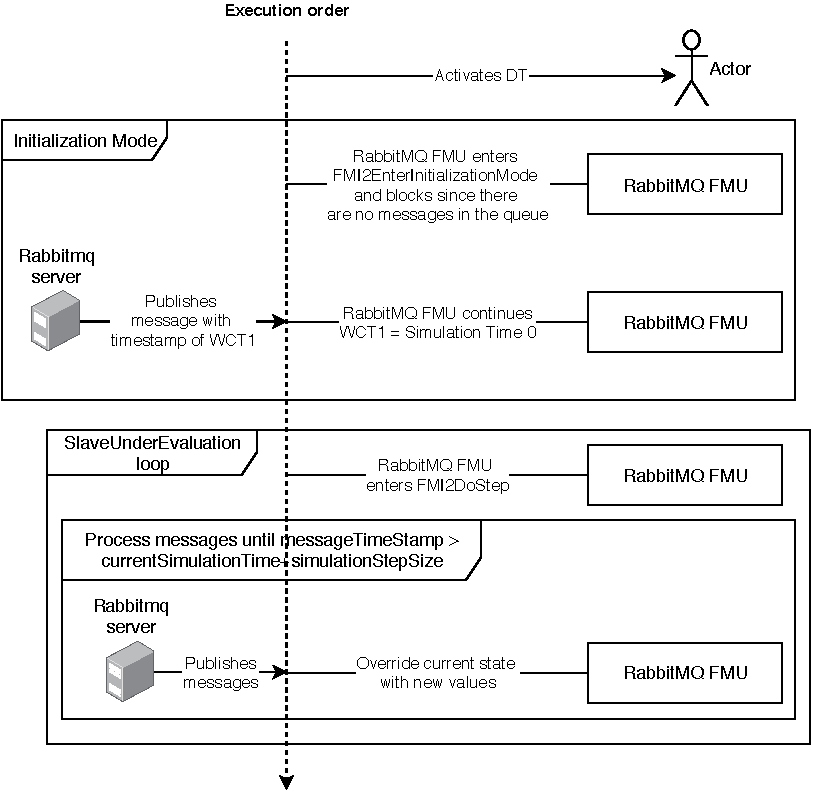
\includegraphics[width=\textwidth]{figures/timehandling.pdf}
  \caption{Time Handling in Simulation View}
  \label{fig:time-handling_simulation-view}
\end{figure}

Invoking the function \texttt{fmi2EnterInitializationMode} on EDB FMU causes it to
block until a message is available.\\
The time stamp of the first message ($WCT1$) received defines $simulationTime0$ and EDB
FMU continues. Thus $WCT1 = simulationTime0$ and a mapping between WCT and simulation time is
establishedcreated. Thus, any subsequent timestamps has $WCT1$ subtracted in order to map
them to $simulationTime$.\\
This also implies that any message with a time stamp of $WCT 0 < WCT1$ are ignored.

Invoking the function \texttt{fmi2DoStep} on EDB FMU causes it to process
messages and keep executing until there is a message with a time stamp defined by
$message\-TimeStamp\-InSimulationTime >= currentSimulationTime +
simulationStepSize$. Such a message is stored in order to use it for the
subsequent \texttt{fmi2DoStep} operation.

%%% Local Variables:
%%% mode: latex
%%% TeX-master: "../rabbitmq-fmu"
%%% End:
